% -*- coding: utf-8 -*-
\chapter{Arquitectura e implementación}
\label{ch:implementacion}

\section{Diseño e implementación de la aplicación}
El diseño se resume en el esquema siguiente, que materializa el hexágono justificado en el Capítulo~\ref{ch:metodologia}. Las figuras~\ref{fig:diagrama-aplicacion} y~\ref{fig:rag-hexagon} lo ilustran: la primera, los bloques desplegados; la segunda, el hexágono del back-end.

\begin{enumerate}[leftmargin=*, itemsep=0.8em, label=\textbf{\arabic*.}]
  \item \textbf{Diseño de la aplicación.}
        La aplicación se organiza en cuatro bloques orquestados con Docker Compose: el front-end en React, Vite, TypeScript y Tailwind CSS; el back-end en FastAPI; PostgreSQL con \texttt{pgvector}; y Ollama para Llama~3.2 y los embeddings. Cada servicio corre en su contenedor. El MVP expone únicamente autenticación, documentos y chat agéntico. La figura~\ref{fig:diagrama-aplicacion} muestra esa composición.

\begin{figure}[htbp]
\centering

\includegraphics[width=\textwidth]{figures/diagrama-aplicacion-agrops.png}
\caption{Diagrama de la aplicación AgroPS: frontend, backend, base de datos e inferencia orquestados con Docker Compose.}
\label{fig:diagrama-aplicacion}
\end{figure}
\end{enumerate}

\section{Back-end, diseño e implementación}
El back-end es la parte de la aplicación encargada de gestionar la lógica de negocio, procesar las consultas y de interactuar para recuperar y almacenar evidencia documental. Actúa como intermediario entre el front-end y las fuentes de información: la base vectorial, el índice léxico y el modelo generativo.

Ha sido construido utilizando Python como lenguaje de programación y FastAPI como marco para construir la API REST. El núcleo RAG no mezcla las reglas de citación con SQLAlchemy ni con Ollama: vive en \texttt{gateway/rag} y se cablea en \texttt{build\_rag\_container}. La figura~\ref{fig:esquema-backend} muestra el esquema de ese back-end: dominio en el centro, aplicación con casos de uso y puertos, y adaptadores en el anillo exterior.

\begin{figure}[htbp]
\centering

\includegraphics[width=\textwidth]{figures/esquema-backend-agrops.png}
\caption{Esquema del back-end AgroPS: dominio en el centro, aplicación con casos de uso y puertos de entrada/salida, y adaptadores en el anillo exterior (API REST, PostgreSQL/\texttt{pgvector}, Ollama y BM25). Los puertos desacoplan la lógica de negocio de la infraestructura.}
\label{fig:esquema-backend}
\end{figure}

La figura~\ref{fig:rag-hexagon} particulariza el mismo diseño en notación hexagonal de puertos y adaptadores.

\definecolor{hexdomain}{HTML}{1A365D}
\definecolor{hexapp}{HTML}{2B6CB0}
\definecolor{hexfw}{HTML}{90CDF4}
\definecolor{hexport}{HTML}{38A169}
\definecolor{hexside}{HTML}{C53030}
\definecolor{hexactor}{HTML}{A0AEC0}

\begin{figure}[htbp]
\centering
\resizebox{\textwidth}{!}{%
\begin{tikzpicture}[
  font=\scriptsize,
  >=Stealth,
  actor/.style={
    regular polygon,
    regular polygon sides=6,
    minimum size=1.28cm,
    inner sep=0pt,
    draw=black!45,
    line width=0.6pt,
    fill=hexactor,
    font=\tiny\bfseries
  },
  portbox/.style={
    draw=hexport!80!black,
    fill=hexport,
    text=white,
    font=\tiny\bfseries,
    inner sep=3.2pt,
    align=center,
    rounded corners=1pt
  },
  sidelab/.style={
    draw=hexside,
    fill=hexside,
    text=white,
    font=\tiny\bfseries,
    inner sep=3.4pt,
    rounded corners=1pt
  }
]
  % --- Tres anillos ---
  \node[
    regular polygon, regular polygon sides=6,
    minimum size=7.35cm, inner sep=0pt,
    draw=hexfw!70!black, line width=0.9pt, fill=hexfw
  ] (fw) at (0,0) {};
  \node[
    regular polygon, regular polygon sides=6,
    minimum size=5.35cm, inner sep=0pt,
    draw=hexapp!70!black, line width=0.9pt, fill=hexapp
  ] (app) at (0,0) {};
  \node[
    regular polygon, regular polygon sides=6,
    minimum size=3.15cm, inner sep=0pt,
    draw=hexdomain!80!black, line width=1.05pt, fill=hexdomain
  ] (dom) at (0,0) {};

  \node[align=center, font=\small\bfseries, text=white] at (0,0.08)
    {Domain\\[-1pt]{\fontsize{6}{7}\selectfont\texttt{rag/domain}}};
  \node[align=center, font=\tiny\bfseries, text=white] at (0,2.05)
    {Application\\[-1pt]{\fontsize{5.5}{6.5}\selectfont\texttt{rag/application}}};
  \node[align=center, font=\tiny\bfseries, text=hexdomain] at (0,3.22)
    {Framework};

  % Puertos y adaptadores (sobre los anillos)
  \node[portbox] (adin) at (-3.05,0.55) {Adapter In};
  \node[portbox] (pin)  at (-2.22,-0.42) {Port In};
  \node[portbox] (uc)   at (-1.88,0.92) {Use case};
  \node[portbox] (pout) at (2.22,-0.42) {Port Out};
  \node[portbox] (adout) at (3.05,0.55) {Adapter Out};

  \node[font=\fontsize{5}{6}\selectfont\ttfamily, text=white, align=center]
    at (-1.70,-1.22) {AnswerQuestion\\HybridRetrieve};
  \node[font=\fontsize{5}{6}\selectfont\ttfamily, text=white, align=center]
    at (1.70,-1.22) {ChunkRepository\\LlmPort · Lexical};

  % --- Driver Side ---
  \node[sidelab] at (-6.95,4.45) {Driver Side};
  \node[actor] (ui) at (-6.95,3.25) {UI};
  \node[align=center, font=\tiny] at (-6.95,2.38) {React / Vite};
  \node[actor] (test) at (-6.95,1.15) {Test};
  \node[align=center, font=\tiny] at (-6.95,0.28) {\texttt{test\_rag\_hexagon}};
  \node[actor] (din) at (-6.95,-0.95) {Int.};
  \node[align=center, font=\tiny] at (-6.95,-1.82) {FastAPI + AgenticRAG};

  \draw[decorate, decoration={brace, amplitude=7pt, raise=1pt}, hexapp, line width=1.1pt]
    (-5.62,3.65) -- (-5.62,-1.55);
  \node[font=\tiny\bfseries, text=hexapp, rotate=90] at (-5.18,1.05) {API};

  \draw[->, thick, hexapp] (ui.east) -- ++(0.32,0) |- (adin.west);
  \draw[->, thick, hexapp] (test.east) -- ++(0.20,0) |- (adin.west);
  \draw[->, thick, hexapp] (din.east) -- ++(0.32,0) |- (adin.west);

  % --- Driven Side ---
  \node[sidelab] at (6.95,4.45) {Driven Side};
  \node[actor] (pers) at (6.95,3.25) {DB};
  \node[align=center, font=\tiny] at (6.95,2.38) {PostgreSQL/\texttt{pgvector}};
  \node[actor] (mock) at (6.95,1.15) {Mock};
  \node[align=center, font=\tiny] at (6.95,0.28) {puertos falsos};
  \node[actor] (dout) at (6.95,-0.95) {Int.};
  \node[align=center, font=\tiny] at (6.95,-1.82) {Ollama · BM25 · reranker};

  \draw[decorate, decoration={brace, amplitude=7pt, mirror, raise=1pt}, hexapp, line width=1.1pt]
    (5.62,3.65) -- (5.62,-1.55);
  \node[font=\tiny\bfseries, text=hexapp, rotate=90] at (5.18,1.05) {SPI};

  \draw[->, thick, hexapp] (adout.east) -- ++(0.35,0) |- (pers.west);
  \draw[->, thick, hexapp] (adout.east) -- ++(0.22,0) |- (mock.west);
  \draw[->, thick, hexapp] (adout.east) -- ++(0.35,0) |- (dout.west);

  % Inversión de dependencias
  \draw[->, line width=1.15pt, hexdomain]
    (5.55,4.05) -- (2.35,2.55);
  \node[font=\tiny\itshape, text=hexdomain, rotate=-28] at (4.25,3.55) {Dependency Inversion};
  \draw[->, line width=1.15pt, hexdomain]
    (-5.55,-3.55) -- (-2.35,-2.55);
  \node[font=\tiny\itshape, text=hexdomain, rotate=-28] at (-4.15,-3.35) {Dependency Inversion};

  \node[align=center, font=\fontsize{6}{7.5}\selectfont, text=black!70]
    at (0,-4.35) {Composition root: \texttt{build\_rag\_container} inyecta adaptadores en los casos de uso.\\
    Fuera del hexágono: JWT, tenants, organizaciones, cuaderno de campo y OpenData.};
\end{tikzpicture}%
}
\caption{Esquema del back-end hexagonal (\texttt{gateway/rag}). El lado conductor entra por \emph{Adapter In} / \emph{Port In}; el lado conducido se conecta por \emph{Port Out} / \emph{Adapter Out}.}
\label{fig:rag-hexagon}
\end{figure}

\begin{table}[htbp]
\centering
\caption{Correspondencia entre anillos del hexágono y paquetes del backend.}
\label{tab:hexagon-packages}
\small
\begin{tabular}{@{}llp{8.6cm}@{}}
\toprule
\textbf{Anillo} & \textbf{Paquete} & \textbf{Contenido verificable} \\
\midrule
Domain & \texttt{rag/domain} & Entidades, \texttt{rrf\_fusion}, \texttt{expand\_agro\_query}, protocolos de puerto \\
Application & \texttt{rag/application} & Casos de uso: \texttt{AnswerQuestion}, \texttt{HybridRetrieve}, \texttt{IngestDocument} \\
Framework / Adapter In & \texttt{routes/*}, \texttt{services/} & FastAPI, \texttt{RAGService}, \texttt{AgenticRAGService} \\
Framework / Adapter Out & \texttt{rag/adapters/outbound} & pgvector, BM25, Ollama, Cross-Encoder \\
Cableado & \texttt{rag/composition.py} & \texttt{build\_rag\_container} (inyección de adaptadores) \\
\bottomrule
\end{tabular}
\end{table}

\subsection{Capa de dominio}
La capa de dominio representa el modelo y las reglas de negocio, abstraída de tecnologías externas a través de las entidades, objetos valor y enumerados. El problema que modela no es un cultivo sobre un mapa, sino la consulta de normativa agrícola con una respuesta fundamentada en fragmentos citables. En esta aplicación se definen las entidades y objetos valor que pueden verse en la figura~\ref{fig:entidades-dominio}, las cuales se presentan a continuación.

\begin{figure}[htbp]
\centering

\includegraphics[width=\textwidth]{figures/entidades-dominio-rag.png}
\caption{Entidades y objetos valor del dominio RAG: la consulta produce un \texttt{RetrievalBundle} que contiene uno o más \texttt{RetrievedChunk}, cada uno identificable por documento y fuente.}
\label{fig:entidades-dominio}
\end{figure}

\subsection{Entidades}
Como puede verse en la figura~\ref{fig:entidades-backend}, el back-end se articula en torno a cuatro entidades de persistencia. El dominio hexagonal no opera sobre ellas de forma directa: el adaptador PostgreSQL las traduce hacia \texttt{RetrievedChunk}, que es la proyección ya recuperada que viaja hasta la cita en el chat.

\begin{figure}[htbp]
\centering

\includegraphics[width=0.95\textwidth]{figures/entidades-backend-agrops.png}
\caption{Entidades de persistencia del back-end: un \texttt{Tenant} agrupa bases de conocimiento y documentos; cada \texttt{Document} pertenece a una \texttt{KnowledgeBase} y se fragmenta en \texttt{Chunk} con su \texttt{Embedding}.}
\label{fig:entidades-backend}
\end{figure}

\texttt{Chunk} se trata de, junto con los documentos, la entidad más importante del dominio, la cual representa un fragmento de normativa o de manual ya extraído, con características como su posición dentro del fichero, un titular, un resumen, el texto completo y el documento al que pertenece. Asociado a cada fragmento se almacena además un \texttt{Embedding}: el modelo que lo generó y el vector de alta dimensión que permite la búsqueda por similitud. Como puede verse, esta entidad es la encargada de almacenar la información más relevante a mostrar como evidencia en el chat: sin ella no hay trazabilidad.

\texttt{Document} es la encargada de almacenar también información muy relevante para la recuperación: representa los ficheros ---PDF, texto u otros tipos MIME--- que contienen los fragmentos. Almacena el nombre original, el tipo MIME, la ruta de almacenamiento, el \texttt{tenant} y la base de conocimiento a la que pertenece, y el propietario. Un documento se fragmenta en uno o más \texttt{Chunk}.

La entidad \texttt{KnowledgeBase} agrupa los documentos que el usuario indexa. En el MVP existe una base por defecto: no hay selector de cooperativas ni de departamentos en la interfaz.

El aislamiento por \texttt{tenant} permanece en persistencia para no mezclar corpus entre cuentas, pero no se gestiona como producto: el usuario ve documentos y chat.

En la capa de dominio hexagonal, \texttt{RetrievedChunk} es esa misma unidad una vez recuperada. Almacena el texto (\texttt{page\_content}), la identidad de \texttt{chunk\_id} y \texttt{document\_id}, el fichero de origen (\texttt{source}), el \texttt{tenant\_id}, la colección (\texttt{knowledge\_base\_id}) y si llegó por vía densa o léxica (\texttt{retrieval\_source}). Los modelos SQLAlchemy no se importan en \texttt{rag/domain}.

La tabla~\ref{tab:entidades-dominio} resume el dominio hexagonal. La tabla~\ref{tab:entidades-persistencia} recoge las entidades de persistencia del monolito que el adaptador PostgreSQL utiliza para materializar ese dominio.

\begin{table}[htbp]
\centering
\caption{Entidades y objetos valor del dominio RAG.}
\label{tab:entidades-dominio}
\small
\begin{tabular}{@{}llp{7.4cm}@{}}
\toprule
\textbf{Tipo} & \textbf{Nombre} & \textbf{Atributos y relaciones} \\
\midrule
Entidad & \texttt{RetrievedChunk} & \texttt{chunk\_id}, \texttt{document\_id}, texto, fuente, \texttt{tenant\_id}, colección, vía densa/léxica. Se identifica por documento y fragmento; alimenta la cita. \\
Objeto valor & \texttt{RetrievalQuery} & Pregunta, \texttt{tenant\_id}, colecciones, estrategia, métrica, rerank y reescritura. Produce un \texttt{RetrievalBundle}. \\
Objeto valor & \texttt{RetrievalBundle} & Consulta reescrita, listas densa y BM25, candidatos RRF, chunks finales y tiempos. Contiene $1..n$ \texttt{RetrievedChunk}. \\
\bottomrule
\end{tabular}
\end{table}

\begin{table}[htbp]
\centering
\caption{Entidades de persistencia del back-end (SQLAlchemy) y sus relaciones principales.}
\label{tab:entidades-persistencia}
\small
\begin{tabular}{@{}llp{6.8cm}@{}}
\toprule
\textbf{Entidad} & \textbf{Atributos principales} & \textbf{Relaciones} \\
\midrule
\texttt{Organization} & identificador, nombre & Interno; no se expone en el MVP. \\
\texttt{Tenant} & identificador, nombre & Aísla el corpus de cada cuenta. \\
\texttt{User} & identificador, nombre, email, hash, activo & Propietario de documentos y conversaciones. \\
\texttt{KnowledgeBase} & identificador, nombre, tenant & Contiene $1..n$ \texttt{Document}. \\
\texttt{Document} & identificador, fichero, MIME, tenant, KB, propietario & Tiene $1..n$ \texttt{Chunk} y versiones. \\
\texttt{Chunk} & identificador, posición, titular, resumen, texto & Pertenece a un \texttt{Document}; tiene \texttt{Embedding}. \\
\texttt{Embedding} & vector, modelo & Pertenece a un \texttt{Chunk}. \\
\texttt{Conversation} & identificador, título, tenant, usuario, KB & Contiene $1..n$ \texttt{Message}. \\
\texttt{Message} & rol, contenido, tokens & Pertenece a una \texttt{Conversation}; cita fuentes. \\
\texttt{MessageSource} & documento, chunk, puntuación & Enlaza un \texttt{Message} con evidencia. \\
\bottomrule
\end{tabular}
\end{table}

\subsection{Objetos valor}
Un objeto valor se trata de un componente inmutable que se utiliza para la creación de las entidades y de las operaciones del dominio. Para las características descritas se definen los objetos valor que se exponen a continuación:

\texttt{RetrievalQuery} representa una consulta. Almacena la pregunta en lenguaje natural, el \texttt{tenant\_id} que acota el aislamiento, las colecciones sobre las que se busca, la estrategia de recuperación, la métrica de distancia y los indicadores de reranking, reescritura de consulta y modo evaluación.

\texttt{RetrievalBundle} agrupa el resultado de una recuperación. Contiene la consulta reescrita, las listas densa y BM25, los candidatos fusionados por RRF, los fragmentos finales y los tiempos de cada etapa. Contiene uno o más \texttt{RetrievedChunk}.

La cita o fuente ---documento, sección y página--- viaja en los metadatos del fragmento. Es inmutable una vez recuperada: no se reescribe al generar la respuesta. Los identificadores de \texttt{tenant}, documento y fragmento viajan como valores dentro de la consulta y del \texttt{RetrievedChunk}; no se reifican en clases propias.

Las reglas puras ---fusión RRF y expansión del léxico agrario--- operan sobre estos objetos en \texttt{rag/domain}, de modo que un cambio de almacén vectorial no redefine qué cuenta como evidencia.

\subsection{Enumerados}
Los enumerados permiten definir una serie de valores fijos con sentido dentro del dominio. Gracias a esto se pueden delimitar valores determinados y reducir la posibilidad de errores en el código. En este proyecto se usan los siguientes:

La estrategia de recuperación se encarga de definir las distintas formas de obtener evidencia, tales como \texttt{dense}, \texttt{bm25}, \texttt{hybrid} y \texttt{hybrid\_rrf}.

El modo del chat en el MVP es RAG agéntico: el orquestador invoca la herramienta \texttt{search\_knowledge\_base} sobre el corpus indexado. La comparación frente a un LLM sin recuperación se reserva al Capítulo~\ref{ch:evaluacion}.

La métrica de distancia fija cómo se compara un vector de consulta con los embeddings persistidos: \texttt{cosine}, \texttt{euclidean}, \texttt{manhattan} e \texttt{inner\_product}.

\subsection{Capa de aplicación}
En la capa de aplicación se encuentran tanto los casos de uso como los puertos, descritos a continuación:

\textbf{Casos de uso.} Se tratan de aquellos que permiten operar sobre las entidades del dominio ---consultar e ingestiar--- sin detalles técnicos de SQL ni de HTTP. \texttt{AnswerQuestion} responde con evidencia; \texttt{HybridRetrieve} recupera de forma densa y léxica y fusiona con RRF; \texttt{IngestDocument} reconstruye el índice léxico e invalida la caché tras indexar un documento. La evaluación cuantitativa no forma parte de la API del MVP.

\textbf{Puertos.} En el caso de esta aplicación, son las interfaces que el dominio necesita del exterior. Los de entrada coinciden con el contrato \texttt{execute} de cada caso de uso, que invocan el front-end y FastAPI a través de \texttt{RAGService}. Los de salida --- \texttt{ChunkRepository}, \texttt{EmbeddingPort}, \texttt{LlmPort}, \texttt{LexicalIndexPort} y \texttt{RerankerPort} --- declaran qué datos se piden ---fragmentos, vectores, texto generado, reordenación--- sin decir cómo obtenerlos. Con ayuda del adaptador PostgreSQL y de Ollama, que se explican a continuación, se consigue la persistencia vectorial, la generación y el reranking.

\subsection{Capa de adaptadores}
Los adaptadores se encargan de conectar la aplicación con el mundo exterior. Como adaptadores de salida están el adaptador PostgreSQL/\texttt{pgvector}, el índice BM25, Ollama y el Cross-Encoder, que implementan los puertos definidos en el dominio. Por otra parte, como adaptador de entrada, está el adaptador API REST, que hace uso de los casos de uso definidos en la capa de aplicación.

\paragraph{Adaptador API REST}
Para desarrollar el adaptador de API REST se hace uso de FastAPI\footnote{\url{https://fastapi.tiangolo.com/}}, un marco de Python para construir APIs a partir de type hints y modelos Pydantic. El adaptador REST se encarga de ofrecer una forma de invocar los casos de uso del dominio, exponiéndolos a través de una interfaz HTTP bajo \texttt{/api/v1}. Las rutas del MVP son las justas para autenticar, indexar documentos y preguntar:

\begin{itemize}[leftmargin=*, itemsep=0.15em]
  \item \texttt{POST /api/v1/auth/register}, \texttt{/login}, \texttt{/logout} y \texttt{GET /me}
  \item \texttt{GET /api/v1/health}
  \item \texttt{GET/POST /api/v1/knowledge/} y \texttt{GET /knowledge/current}
  \item \texttt{GET/POST /api/v1/documents} y \texttt{DELETE /documents/\{id\}}
  \item \texttt{POST /api/v1/chat/}, \texttt{GET /chat/conversations} y \texttt{GET/DELETE /chat/\{id\}}
\end{itemize}

El controlador de chat autentica, acota el corpus de la cuenta y delega en \texttt{AgenticRAGService}. El orquestador planifica la herramienta \texttt{search\_knowledge\_base}; no contiene la fusión RRF, que permanece en el dominio.

\paragraph{Adaptador PostgreSQL}
PostgreSQL\footnote{\url{https://www.postgresql.org/}} se trata de un sistema de base de datos relacional de código abierto, con décadas de desarrollo activo. Se sitúa como una de las soluciones más fiables en el mundo de las bases de datos y es ampliamente utilizado por desarrolladores y empresas. En este proyecto se extiende con \texttt{pgvector}\footnote{\url{https://github.com/pgvector/pgvector}}, que añade tipos vectoriales y búsqueda por similitud.

Por otra parte, SQLAlchemy\footnote{\url{https://docs.sqlalchemy.org/}} es el ORM con el que el back-end declara las tablas y ejecuta consultas asíncronas. Su uso queda confinado a los adaptadores de salida: el caso de uso solo recibe \texttt{RetrievedChunk}.

En este proyecto, para la implementación del adaptador PostgreSQL, \texttt{PgvectorChunkRepository} implementa el puerto \texttt{ChunkRepository}: embebe la pregunta, ejecuta la búsqueda por vecinos próximos ---índice HNSW, métrica configurable--- y filtra por organización y colecciones. Mediante SQLAlchemy y las sentencias sobre \texttt{pgvector} se realizan la recuperación densa de fragmentos y, en la ingesta, la persistencia de documento, \texttt{chunk} y vector.

\paragraph{Adaptadores de inferencia y léxico}
\texttt{OllamaLlmAdapter} y \texttt{OllamaEmbeddingAdapter} implementan \texttt{LlmPort} y \texttt{EmbeddingPort} contra Llama~3.2 y \texttt{nomic-embed-text}, servidos en local por Ollama\footnote{\url{https://ollama.com/}}. \texttt{Bm25LexicalIndex} cubre la búsqueda léxica y su reconstrucción tras la ingesta. \texttt{CrossEncoderReranker} reordena candidatos cuando la estrategia lo pide. Sustituir el modelo o la base se reduce a cambiar el adaptador y el composition root.

El pipeline híbrido permanece denso + BM25 + RRF, con reranking opcional. Los guardrails envuelven el ciclo pregunta--respuesta: ámbito por \texttt{tenant\_id} y colección, prompt de no invención y, en auditoría, marcas de contexto vacío, alucinación y PII.

\section{Front-end, diseño e implementación}
El front-end es la capa de presentación con la que el técnico agrícola interactúa: autenticación, gestión documental, chat con citas y laboratorio de evaluación. Se ha construido con TypeScript, React~19, Vite y Tailwind CSS, siguiendo la misma idea hexagonal que el back-end: el dominio de la interfaz no conoce \texttt{axios} ni el DOM concreto; los adaptadores HTTP y React cablean casos de uso y servicios. La figura~\ref{fig:esquema-frontend} resume ese diseño.

\begin{figure}[htbp]
\centering

\includegraphics[width=\textwidth]{figures/esquema-frontend-agrops.png}
\caption{Diagrama del front-end AgroPS: dominio en el centro, aplicación con casos de uso y puertos, y adaptadores HTTP (API REST) y React (UI) en el anillo exterior.}
\label{fig:esquema-frontend}
\end{figure}

\subsection{Capa de dominio}
En cuanto al dominio del front-end, se trabaja con las mismas entidades conceptuales que el back-end, traducidas a TypeScript en \texttt{frontend/agrops/src/types}. Los DTO que devuelve la API REST ---\texttt{DocumentItem}, \texttt{Message}, \texttt{Conversation}, \texttt{ChatResponse}--- reflejan el vocabulario del servidor. Los objetos valor de la UI (\texttt{ChatRequest}, \texttt{ContextChunk}, \texttt{RetrievalInfo}) empaquetan una operación concreta sin identidad persistente propia. Los enumerados \texttt{rag\_mode} y \texttt{MessageRole} acotan el comportamiento del chat. El dominio de la interfaz no importa SQLAlchemy ni FastAPI.

\subsection{Capa de aplicación}
En la capa de aplicación se encuentran tanto los casos de uso como los puertos. Los \textbf{casos de uso} se implementan como servicios (\texttt{auth.service}, \texttt{document.service}, \texttt{chat.service}, \texttt{evaluation.service}): registran e inician sesión, listan y suben documentos, envían preguntas al RAG y lanzan evaluaciones. Los \textbf{puertos de entrada} son las páginas y \emph{hooks} React que invocan esos servicios. Los \textbf{puertos de salida} son las interfaces HTTP (\texttt{api.ts}) que declaran qué datos se piden al back-end sin fijar \texttt{axios} en cada componente.

\subsection{Capa de adaptadores}
En la capa de adaptadores se definen las conexiones con el exterior del front-end:

\paragraph{Adaptador HTTP}
Implementa el puerto de salida y gestiona la comunicación con el back-end mediante llamadas HTTP a \texttt{/api/v1}, adjuntando el JWT y traduciendo errores de autenticación.

\paragraph{Adaptador React}
Organiza vistas (\texttt{pages/}), componentes reutilizables, React Router y TanStack Query. Incluye \textbf{internacionalización (i18n)} con ficheros \texttt{src/i18n/locales} al estilo \emph{i18next}\footnote{\url{https://www.i18next.com/}}: el selector de idioma en Ajustes conmuta la interfaz entre español e inglés.

\subsection{Flujo end-to-end de una consulta}
La figura~\ref{fig:flujo-e2e} describe el recorrido de una pregunta. El usuario formula la consulta en el chat React. FastAPI autentica, resuelve el corpus de la cuenta y persiste el mensaje. El adaptador de entrada delega en \texttt{AgenticRAGService}, que invoca \texttt{search\_knowledge\_base}. La recuperación ejecuta búsqueda densa (\texttt{pgvector}) y léxica (BM25) y fusiona con RRF. El generador (Llama~3.2 vía Ollama) recibe el contexto anclado y devuelve el texto con documento y página. La interfaz muestra la respuesta y las fuentes. Un fallo de evidencia se declara; no se inventa.

\begin{figure}[htbp]
\centering

\includegraphics[width=\textwidth]{figures/flujo-e2e-agrops.png}
\caption{Flujo end-to-end de una consulta en AgroPS: de la pregunta en el chat a la respuesta citada, pasando por FastAPI, la aplicación RAG, la recuperación híbrida y la generación local.}
\label{fig:flujo-e2e}
\end{figure}

\section{Capturas del prototipo AgroPS}

Las figuras siguientes documentan las funcionalidades principales del MVP frente al tribunal: autenticación implícita en el panel, gestión documental, asistente RAG, visualización del espacio de embeddings, organización multi-tenant y orquestación del pipeline. Un guion completo de capturas adicionales (evaluación, HITL, tools, landing) se mantiene en \texttt{docs/CAPTURAS\_UI.md}.

\begin{figure}[htbp]
\centering

\includegraphics[width=\textwidth]{figures/ui-documentos.png}
\caption{Vista de documentos: listado del corpus por organización, estado de indexado y alta de ficheros.}
\label{fig:ui-docs}
\end{figure}

\begin{figure}[htbp]
\centering

\includegraphics[width=\textwidth]{figures/ui-ingesta.png}
\caption{Flujo de ingesta documental en el prototipo: carga y preparación del material para chunking y embeddings.}
\label{fig:ui-ingesta}
\end{figure}

\begin{figure}[htbp]
\centering

\includegraphics[width=\textwidth]{figures/ui-chat.png}
\caption{Asistente RAG agéntico: pregunta en lenguaje natural, respuesta anclada y evidencia recuperada (fuentes).}
\label{fig:ui-chat}
\end{figure}

\begin{figure}[htbp]
\centering

\includegraphics[width=\textwidth]{figures/ui-grafo.png}
\caption{Visualización del espacio de embeddings (proyección tipo grafo/UMAP). Es una ayuda exploratoria; el chat no recorre un grafo de conocimiento.}
\label{fig:ui-grafo}
\end{figure}

\begin{figure}[htbp]
\centering

\includegraphics[width=\textwidth]{figures/ui-organizacion.png}
\caption{Gestión de organización: selección de cooperativa/empresa, departamentos y contexto multi-tenant del corpus.}
\label{fig:ui-org}
\end{figure}

\section{Alcance del prototipo}
El MVP opera sobre texto y embeddings persistidos. El corpus puede proceder de PDF con OCR, pero retrieval, generación y evaluación son textuales. La interfaz incluye un laboratorio de evaluación (banco, experimentos y auditoría) como herramienta operativa del prototipo; las tablas del Capítulo~\ref{ch:evaluacion} se reportan sobre el banco versionado, no como certificación de un entorno productivo.

\section{Pipeline híbrido de recuperación (detalle de implementación)}
El chat de demostración no recorre un grafo de conocimiento. El caso de uso \texttt{HybridRetrieve} concatena, cuando procede, cuatro listas de candidatos y las fusiona con Reciprocal Rank Fusion (RRF, $k=60$): búsqueda densa en \texttt{pgvector} (similitud coseno sobre \texttt{nomic-embed-text}), búsqueda léxica BM25 por tenant, y las mismas dos vías sobre la consulta expandida con un léxico agrario (sinónimos y formas de cultivo, ayuda, plaga, recinto). Si la pregunta supera un umbral de complejidad (\texttt{should\_rewrite\_query}), un LLM reescribe la consulta; esa reescritura no se aplica a todas las preguntas cortas de hecho directo.

El algoritmo de respuesta (\texttt{AnswerQuestion}) orquesta ese retrieve y la generación: con la pregunta $q$, el historial $H$ y el tenant $t$, recupera el top-$k$ de fragmentos, abstiene con plantilla \emph{out-of-knowledge} si no hay evidencia (sin llamar al LLM) y, en caso contrario, construye un prompt de sistema con el contexto documental recortado, invoca Llama~3.2 vía Ollama y devuelve la respuesta $a$ junto con las fuentes citables $C$. El modo \texttt{hybrid} del API sigue ese camino fijo; el modo \texttt{agentic} añade un grafo LangGraph (planificar herramientas, recuperar, puntuar relevancia y reescribir como máximo una vez) que, cuando busca en la base de conocimiento, reutiliza el mismo recuperador híbrido. La figura~\ref{fig:respuesta-rag} resume ambos caminos; la evaluación cuantitativa del Capítulo~\ref{ch:evaluacion} mide el híbrido fijo.

\begin{figure}[htbp]
\centering
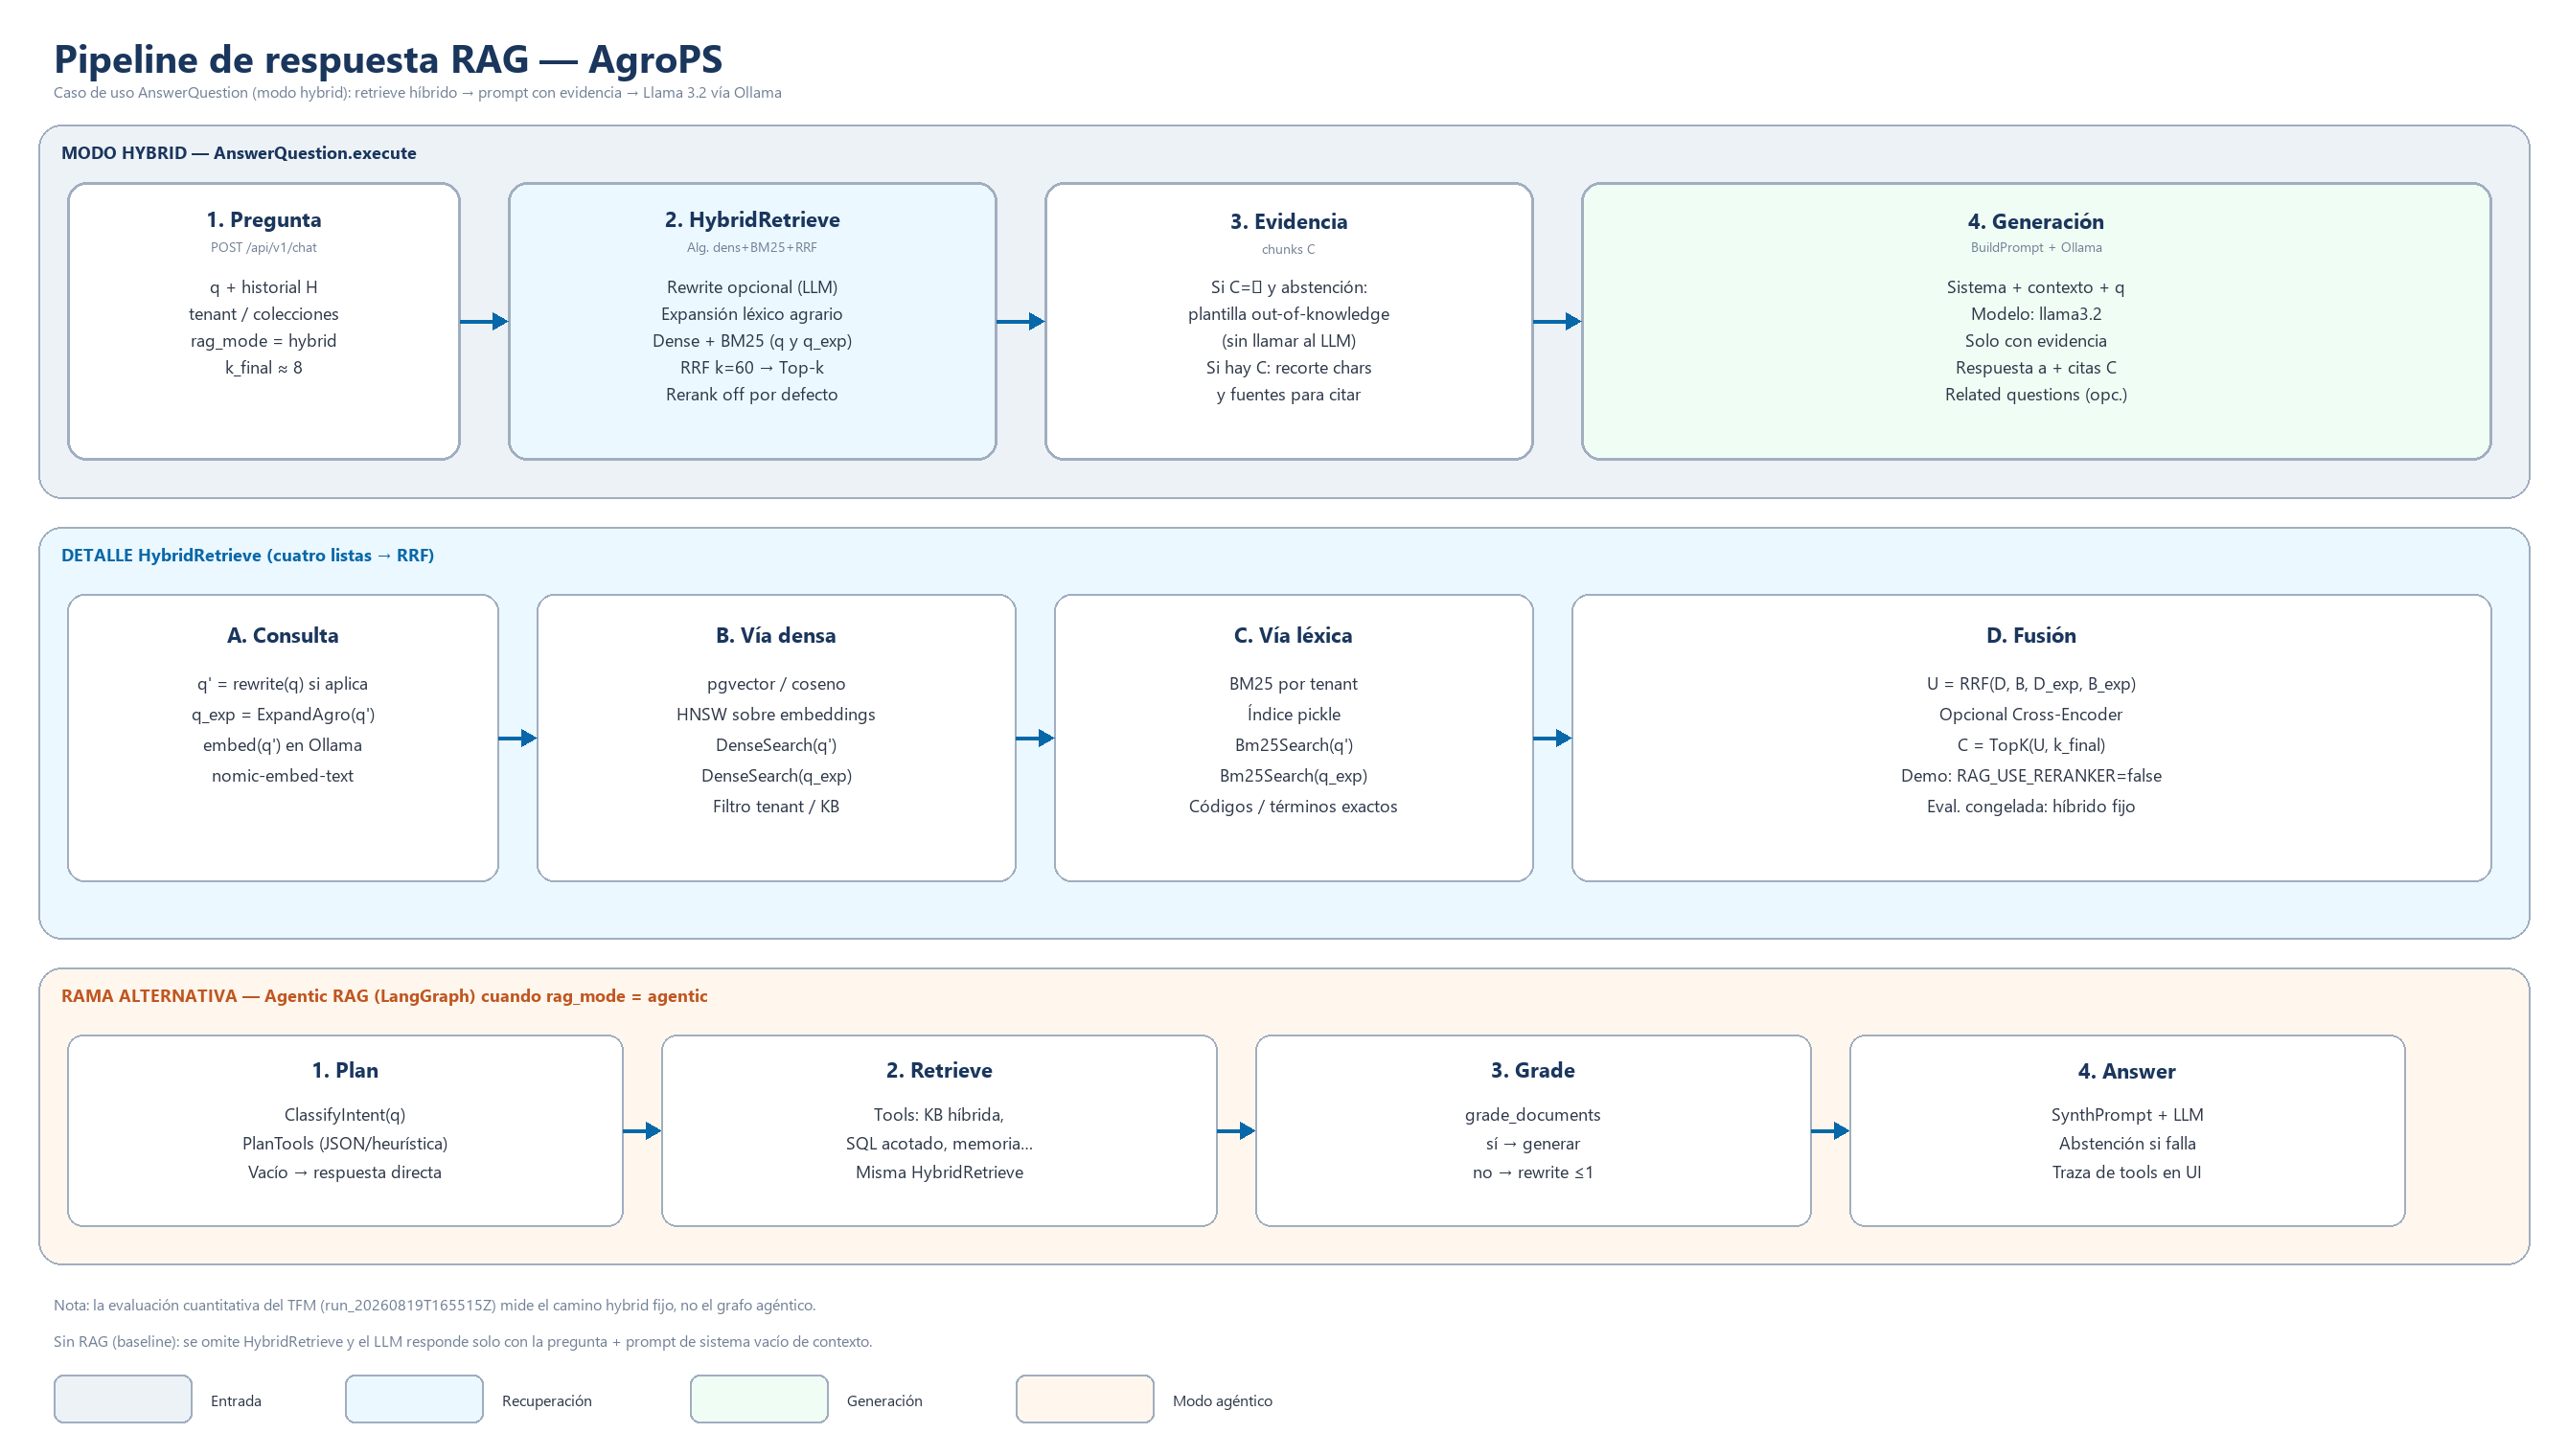
\includegraphics[width=\textwidth]{figures/diagrama-respuesta-rag.png}
\caption{Pipeline de respuesta RAG en AgroPS: camino \texttt{hybrid} (\texttt{AnswerQuestion} + dens+BM25+RRF + generación) y rama alternativa \texttt{agentic} (LangGraph).}
\label{fig:respuesta-rag}
\end{figure}

El reranker \texttt{BAAI/bge-reranker-v2-m3} está cableado como adaptador, pero la variable \texttt{RAG\_USE\_RERANKER} vale \texttt{false} en la demo: las ablaciones de laboratorio mostraron que cargar el Cross-Encoder dispara la latencia (decenas de segundos) y puede hundir Recall@1. El contexto que llega al generador es, por tanto, el top-$k$ fusionado por RRF, recortado a unos 1400 caracteres por fragmento, con $k$ final 8 en el chat.

La fachada \texttt{AgenticRAGService} orquesta un grafo LangGraph: el nodo \texttt{generate\_query\_or\_respond} decide si llamar a herramientas (corpus híbrido, SQL acotado o memoria) o responder directo; tras recuperar, \texttt{grade\_documents} puntúa relevancia y, si falla, \texttt{rewrite\_question} reintenta una vez. El planificador pide JSON a Ollama y, si el parseo falla, cae a pistas léxicas. Las búsquedas invocan el mismo \texttt{\_search} híbrido. El modo \texttt{hybrid} del API omite el grafo y llama directamente a \texttt{RAGService.answer}.

Los algoritmos~\ref{alg:rag-hibrido}, \ref{alg:hybrid-retrieve} y \ref{alg:rag-agentic} formalizan, respectivamente, la respuesta híbrida end-to-end, la recuperación denso+BM25+RRF y el camino agéntico (LangGraph) del chat. La tubería de indexación se formaliza en los algoritmos~\ref{alg:rag-ingest}, \ref{alg:extract-pdf}, \ref{alg:split-chunks} y \ref{alg:embed-store}.

\begin{algorithm}[htbp]
\caption{Respuesta RAG híbrida (modo \texttt{hybrid})}
\label{alg:rag-hibrido}
\begin{algorithmic}[1]
\Require Pregunta $q$, historial $H$, tenant $t$, parámetros $k_{\mathrm{ret}}, k_{\mathrm{final}}$, flags de reescritura y rerank
\Ensure Respuesta $a$ y fragmentos citados $C$
\State $C,\,q' \gets \textsc{HybridRetrieve}(q,t)$ \Comment{Alg.~\ref{alg:hybrid-retrieve}}
\If{$C = \emptyset$ \textbf{and} abstención rápida activa}
  \State \Return plantilla \emph{out-of-knowledge} (sin llamar al LLM)
\EndIf
\State $P \gets \textsc{BuildPrompt}(q, H, C)$ \Comment{sistema + contexto documental + usuario}
\State $a \gets \textsc{Generate}(P)$ \Comment{LLM local vía Ollama}
\State \Return $a,\,C$
\end{algorithmic}
\end{algorithm}

\begin{algorithm}[htbp]
\caption{Recuperación híbrida dens+BM25+RRF}
\label{alg:hybrid-retrieve}
\begin{algorithmic}[1]
\Require Pregunta $q$, tenant $t$
\Ensure Lista ordenada de chunks $C$ y consulta efectiva $q'$
\State $q' \gets q$
\If{\textsc{ShouldRewrite}($q$)}
  \State $q' \gets \textsc{RewriteWithLLM}(q)$ \Comment{opcional; no en todas las consultas cortas}
\EndIf
\State $q_{\mathrm{exp}} \gets \textsc{ExpandAgroLexicon}(q')$ \Comment{sinónimos de cultivo, ayuda, plaga\ldots}
\State $D \gets \textsc{DenseSearch}(\mathrm{embed}(q'), t, k_{\mathrm{ret}})$ \Comment{pgvector / coseno}
\State $B \gets \textsc{Bm25Search}(q', t, k_{\mathrm{bm25}})$
\State $D_{\mathrm{exp}} \gets \textsc{DenseSearch}(\mathrm{embed}(q_{\mathrm{exp}}), t, k_{\mathrm{ret}})$
\State $B_{\mathrm{exp}} \gets \textsc{Bm25Search}(q_{\mathrm{exp}}, t, k_{\mathrm{bm25}})$
\State $U \gets \textsc{RRF}(D, B, D_{\mathrm{exp}}, B_{\mathrm{exp}};\, k_{\mathrm{rrf}}{=}60)$
\If{rerank activo}
  \State $U \gets \textsc{CrossEncoderRerank}(q', U)$
\EndIf
\State $C \gets \textsc{TopK}(U, k_{\mathrm{final}})$
\State \Return $C,\,q'$
\end{algorithmic}
\end{algorithm}

\begin{algorithm}[htbp]
\caption{Respuesta Agentic RAG (LangGraph)}
\label{alg:rag-agentic}
\begin{algorithmic}[1]
\Require Pregunta $q$, historial $H$, tenant $t$, $\textit{maxRewrites}$
\Ensure Respuesta $a$, traza de tools y chunks $C$
\State $q_{\mathrm{act}} \gets q$;\; $r \gets 0$;\; $C \gets \emptyset$
\State $\textit{intent} \gets \textsc{ClassifyIntent}(q)$
\State $\textit{plan} \gets \textsc{PlanTools}(q_{\mathrm{act}}, \textit{intent})$ \Comment{heurística (rápido) o LLM JSON}
\If{$\textit{plan} = \emptyset$}
  \State $a \gets \textsc{Generate}(\textsc{SynthPrompt}(\textit{intent}, \emptyset), q, H)$
  \State \Return $a$ \Comment{saludo / respuesta directa sin retrieve}
\EndIf
\Repeat
  \State Ejecutar cada tool de $\textit{plan}$ (KB híbrida, SQL, memoria, inventario\ldots)
  \State $C,\,\textit{ctx} \gets$ evidencia acumulada
  \If{el plan usó búsqueda documental}
    \State $\textit{grade} \gets \textsc{Grade}(q, \textit{ctx})$ \Comment{heurística o LLM binario}
  \Else
    \State $\textit{grade} \gets \texttt{yes}$
  \EndIf
  \If{$\textit{grade} = \texttt{no}$ \textbf{and} $r < \textit{maxRewrites}$}
    \State $q_{\mathrm{act}} \gets \textsc{RewriteQuestion}(q_{\mathrm{act}})$;\; $r \gets r+1$
    \State $\textit{plan} \gets$ plan de reintento (p.\ ej.\ \texttt{search\_knowledge\_base})
  \EndIf
\Until{$\textit{grade} = \texttt{yes}$ \textbf{or} $r \ge \textit{maxRewrites}$}
\If{$\textit{grade} = \texttt{no}$ \textbf{and} abstención rápida}
  \State \Return plantilla \emph{out-of-knowledge}
\EndIf
\State $a \gets \textsc{Generate}(\textsc{SynthPrompt}(\textit{intent}, \textit{ctx}), q, H)$
\State \Return $a,\,C$
\end{algorithmic}
\end{algorithm}

Los embeddings se calculan sobre el campo \texttt{content} del chunk; el retriever denso y BM25 puntúan la concatenación headline + summary + content. Esa asimetría es una limitación del prototipo: el vector no representa exactamente el texto que se busca. Los vectores Nomic (~768 dimensiones) se almacenan en una columna de 4096 con relleno de ceros, restricción del esquema pgvector heredado.

Esta descripción justifica, frente al tribunal, qué hay de RAG ``de libro'' (Lewis et al., 2020) y qué es ingeniería del MVP: fusión híbrida real, orquestación LangGraph sobre esas mismas herramientas, grafo de conocimiento solo como visualización UMAP, evaluación textual.

\section{Ingesta documental, OCR y persistencia}
\label{sec:ingesta-rag}

La ingesta es el proceso que transforma un fichero subido por el usuario en unidades recuperables: filas \texttt{chunks} (texto) y \texttt{embeddings} (vectores), más un índice léxico BM25 por tenant. En el monolito, el camino vivo es \texttt{POST /api/v1/documents} $\rightarrow$ almacenamiento local $\rightarrow$ tarea asíncrona \texttt{ingest\_uploaded\_document} $\rightarrow$ \texttt{reindex\_embeddings} / \texttt{ensure\_document\_chunks} $\rightarrow$ caso de uso hexagonal \texttt{IngestDocument} (rebuild BM25 e invalidación de caché). La extracción, el cortado y el embedding viven en la capa \texttt{services/}; el hexágono RAG solo cierra la vía léxica. La figura~\ref{fig:ingesta-rag} resume ese flujo.

\begin{figure}[htbp]
\centering
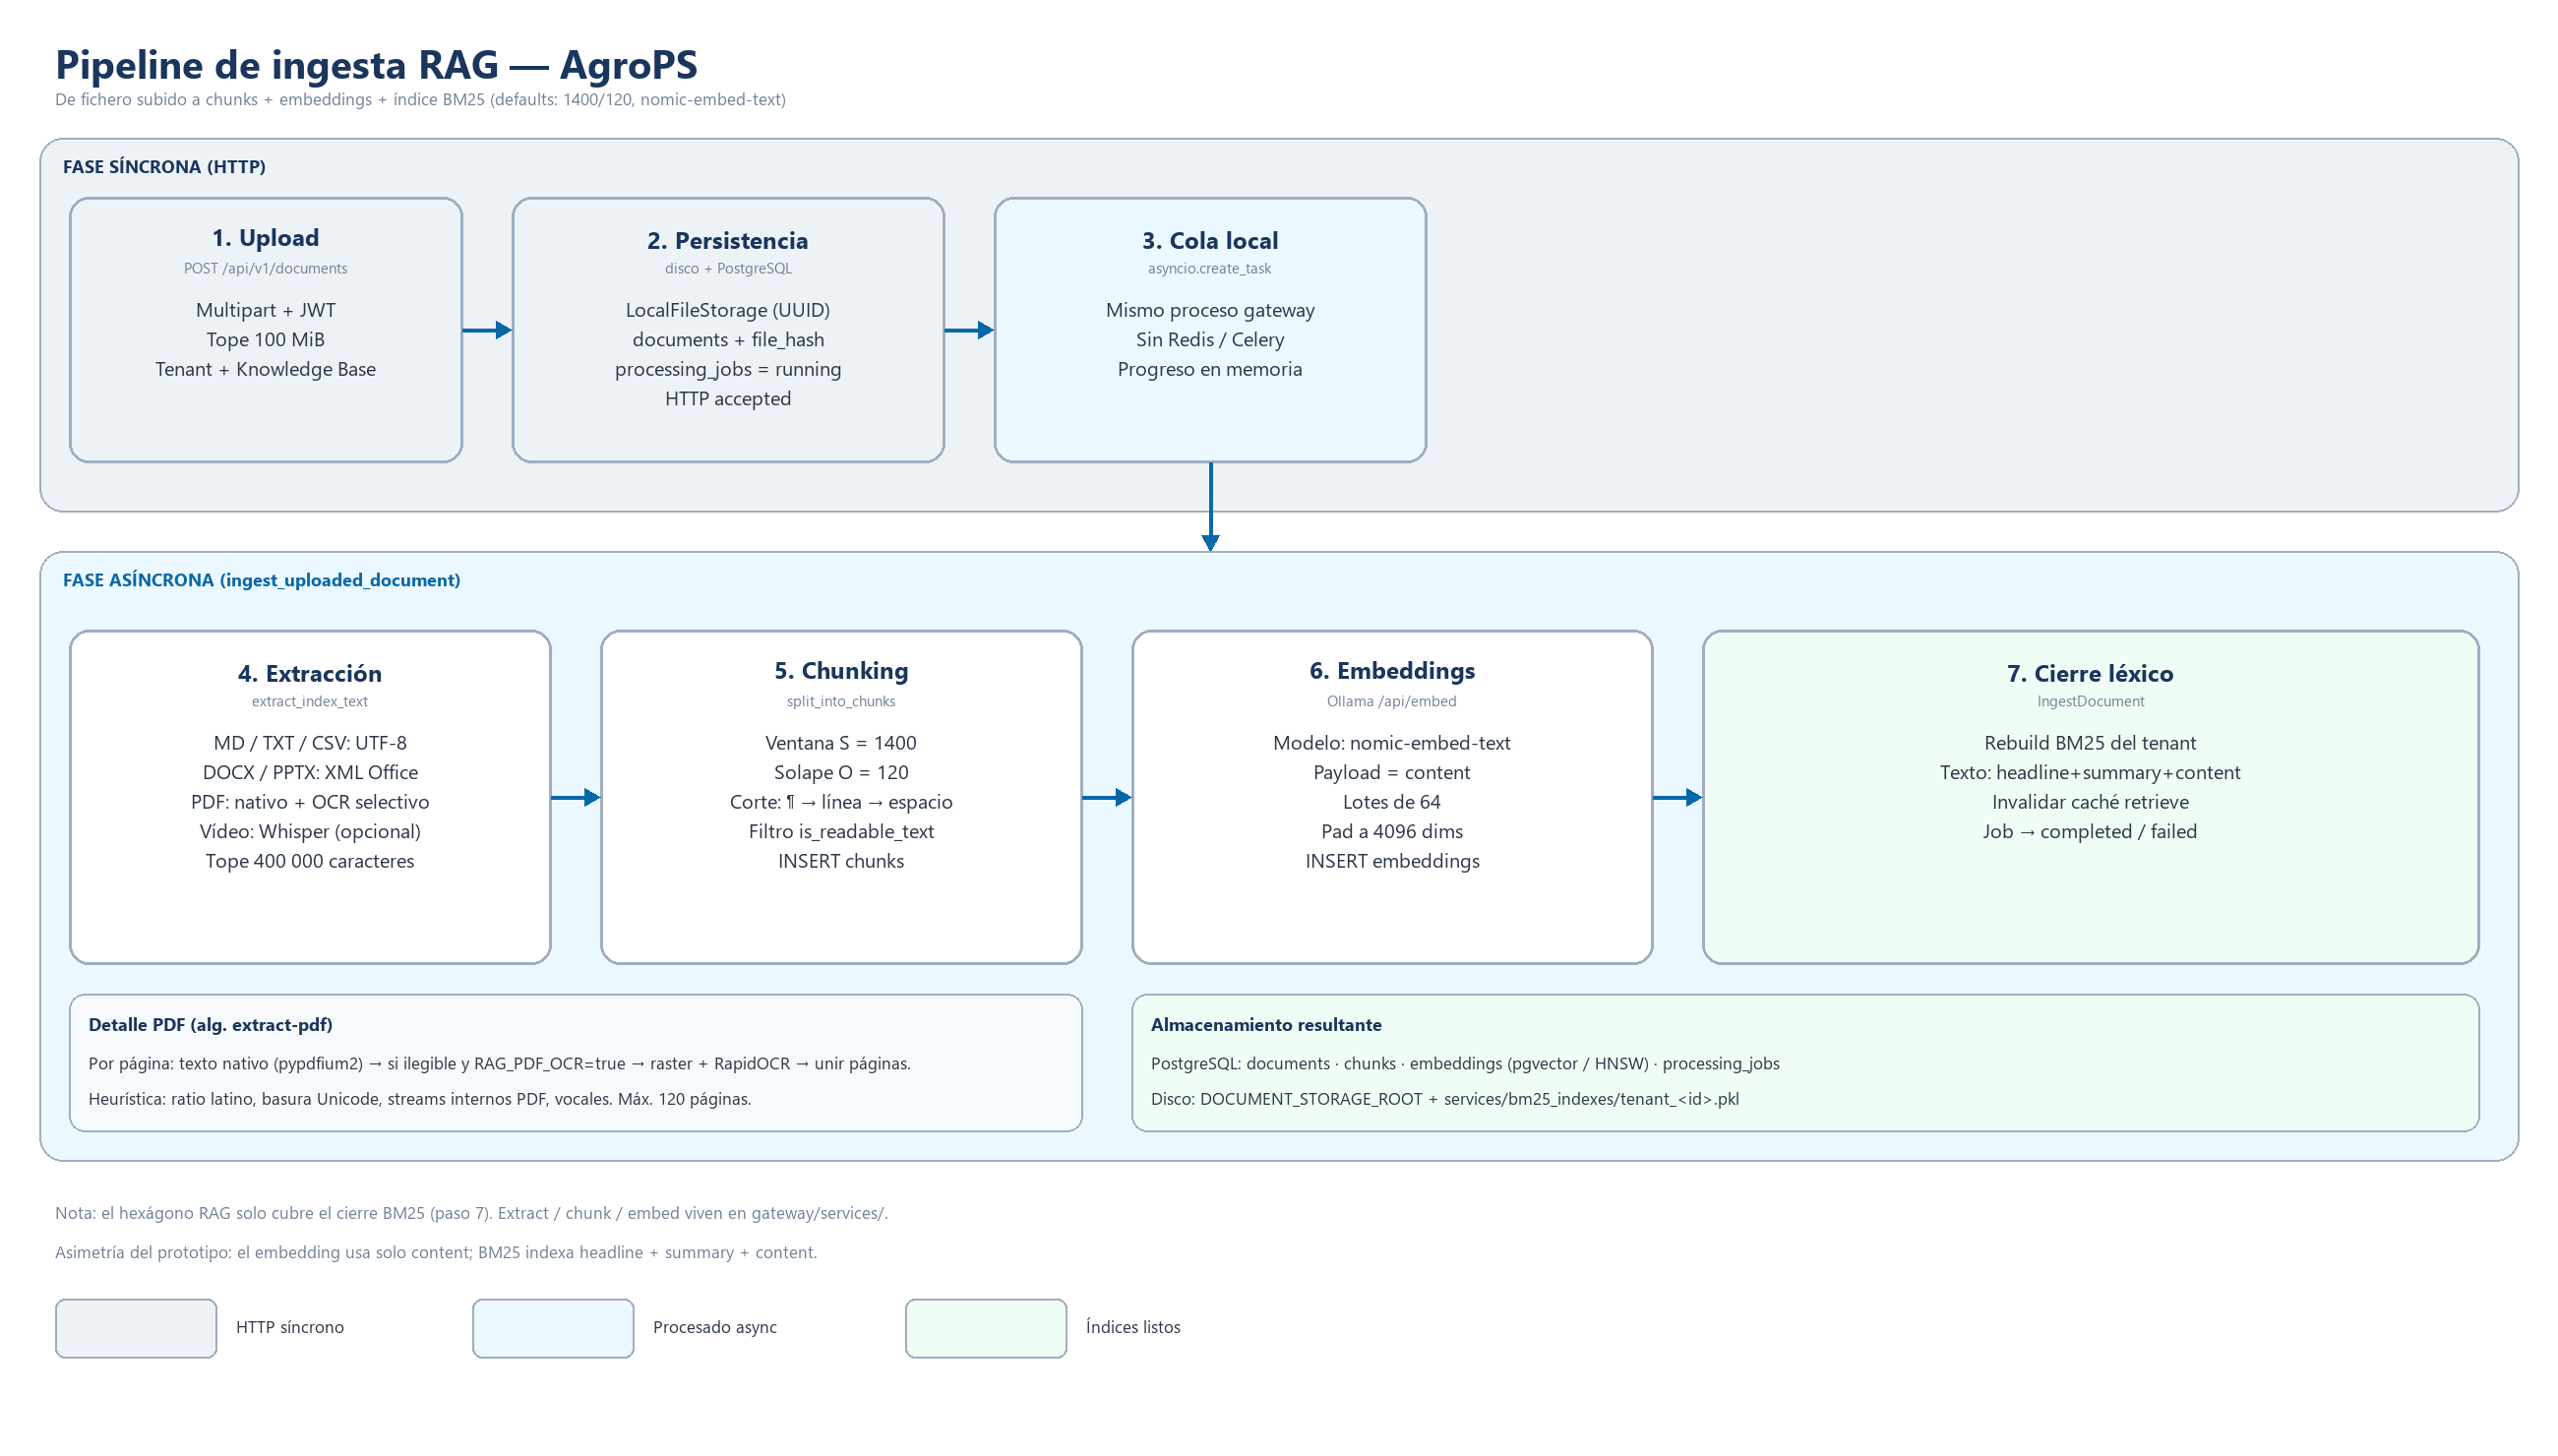
\includegraphics[width=\textwidth]{figures/diagrama-ingesta-rag.png}
\caption{Pipeline de ingesta RAG en AgroPS: aceptación HTTP síncrona, extracción tipada (con OCR selectivo en PDF), fragmentación 1400/120, embeddings densos y reconstrucción BM25 del tenant.}
\label{fig:ingesta-rag}
\end{figure}

\subsection*{Fase A --- Aceptación HTTP (síncrona)}
El usuario autenticado elige organización (tenant) y base de conocimiento. El cuerpo multipart se lee en memoria con tope \texttt{MAX\_UPLOAD\_BYTES} (100\,MiB). \texttt{LocalFileStorage.save\_bytes} escribe el binario bajo \texttt{DOCUMENT\_STORAGE\_ROOT}/\{tenant\}/\{kb\}/\{uuid\}\_\{filename\}. Se insertan \texttt{documents} (incl.\ \texttt{file\_hash} SHA-256, que se persiste pero \textbf{no} deduplica) y \texttt{processing\_jobs} con estado \texttt{running}. La API responde \texttt{accepted} y encola \texttt{asyncio.create\_task} (mismo proceso; no hay cola Redis).

\subsection*{Fase B --- Extracción tipada}
\texttt{extract\_index\_text} despacha por extensión/MIME: texto plano y Markdown (UTF-8, tope $400{,}000$ caracteres); DOCX/PPTX vía XML del ZIP Office; PDF con \texttt{extract\_pdf\_text} (Alg.~\ref{alg:extract-pdf}); vídeo/audio con Whisper. En PDF, cada página obtiene primero texto nativo (pypdfium2). Si \texttt{RAG\_PDF\_OCR} está activo y el texto no supera \texttt{is\_readable\_text} (ratio latino, basura Unicode, ausencia de vocales, detección de streams internos), se rasteriza a escala \texttt{RAG\_PDF\_OCR\_SCALE} y se aplica RapidOCR. El píxel se descarta tras la transcripción: no hay razonamiento visual.

\subsection*{Fase C --- Fragmentación}
\texttt{split\_into\_chunks} (Alg.~\ref{alg:split-chunks}) normaliza saltos de línea y corta ventanas de tamaño $S$ (por defecto $1400$) con solape $O$ ($120$), preferiendo cortar en \texttt{\textbackslash n\textbackslash n}, luego \texttt{\textbackslash n}, luego espacio, siempre que el corte caiga al menos al $40\%$ de $S$. Cada pieza legible ($\ge 24$ caracteres según la misma heurística) se persiste como \texttt{Chunk}: \texttt{position}, \texttt{headline} (primera línea, máx.\ 200), \texttt{summary} (primeros 280 caracteres) y \texttt{content} (cuerpo completo). Si ya existían chunks legibles y no hay \texttt{force\_rebuild}, se reutilizan; si el muestreo parece corrupto, se borran embeddings+chunks y se reextrae.

\subsection*{Fase D --- Embedding y cierre léxico}
Para el modelo por defecto (\texttt{nomic-embed-text}), se embebe solo el \texttt{content} en lotes de tamaño \texttt{RAG\_EMBED\_BATCH\_SIZE} (64). Los vectores se rellenan (\emph{pad}) a 4096 dimensiones y se insertan en \texttt{embeddings} con unicidad $(chunk\_id, model)$. Tras indexar, \texttt{IngestDocument} invalida y reconstruye el BM25 del tenant (texto indexado $=$ headline + summary + content) e invalida la caché de retrieval. Esa asimetría embedding/BM25 es una limitación del prototipo (el vector no representa exactamente el texto que BM25 puntúa).

Los algoritmos~\ref{alg:rag-ingest}--\ref{alg:embed-store} formalizan el pipeline completo. Un error de OCR (``0'' vs ``O'' en una tabla de importes) se propaga al vector y al generador: las fallas de tablas del Capítulo~\ref{ch:evaluacion} empiezan aquí.

\begin{algorithm}[htbp]
\caption{Ingesta RAG end-to-end (\texttt{ingest\_uploaded\_document})}
\label{alg:rag-ingest}
\begin{algorithmic}[1]
\Require Fichero $F$, tenant $t$, base de conocimiento $b$, modelo de embedding $m$, flags $\textit{force}$
\Ensure Filas \texttt{chunks}/\texttt{embeddings}, índice BM25 de $t$, job en estado final
\State $p \gets \textsc{SaveBytes}(F, t, b)$ \Comment{disco: UUID + nombre seguro}
\State $h \gets \textsc{SHA256}(F)$
\State $d \gets \textsc{InsertDocument}(p, h, t, b)$;\; $j \gets \textsc{InsertJob}(d, \texttt{running})$
\State Responder HTTP \texttt{accepted}; encolar tarea asíncrona
\State $\textit{stage} \gets \texttt{extract}$
\State $n \gets \textsc{EnsureDocumentChunks}(d, \textit{force})$ \Comment{Alg.~\ref{alg:split-chunks} tras extracción}
\State $\textsc{EmbedAndStore}(d, t, b, m)$ \Comment{Alg.~\ref{alg:embed-store}}
\State $\textsc{RebuildBm25}(t)$;\; $\textsc{InvalidateRetrievalCache}(t)$
\State Marcar $j$ como \texttt{completed} (o \texttt{failed} si alguna fase lanza error)
\State \Return $n$ fragmentos indexados
\end{algorithmic}
\end{algorithm}

\begin{algorithm}[htbp]
\caption{Extracción de texto PDF (nativo + OCR selectivo)}
\label{alg:extract-pdf}
\begin{algorithmic}[1]
\Require Bytes PDF $B$, $\textit{maxPages}$, $\textit{maxChars}$, flag OCR
\Ensure Texto plano $T$ (truncado a $\textit{maxChars}$)
\State $P \gets \textsc{OpenPdf}(B)$;\; $L \gets \emptyset$
\For{$i \gets 0$ \textbf{to} $\min(|P|, \textit{maxPages})-1$}
  \State $n \gets \textsc{NativePageText}(P_i)$
  \If{OCR activo \textbf{and} $\neg\,\textsc{IsReadable}(n)$}
    \State $s \gets \textsc{RapidOcr}(\textsc{Rasterize}(P_i, \textit{scale}))$
    \If{$\textsc{IsReadable}(s)$ \textbf{or} $\textsc{LatinRatio}(s) > \textsc{LatinRatio}(n)$}
      \State $c \gets s$
    \ElsIf{$\textsc{IsReadable}(n;\,\textit{minChars}{=}12)$}
      \State $c \gets n$
    \Else
      \State \textbf{continue} \Comment{página descartada}
    \EndIf
  \ElsIf{$\textsc{IsReadable}(n;\,\textit{minChars}{=}12)$}
    \State $c \gets n$
  \Else
    \State \textbf{continue}
  \EndIf
  \State $L \gets L \cup \{c\}$
\EndFor
\State \Return truncar$(\textsc{Join}(L,\texttt{\textbackslash n\textbackslash n}),\,\textit{maxChars})$
\end{algorithmic}
\end{algorithm}

\begin{algorithm}[htbp]
\caption{Fragmentación con solape (\texttt{split\_into\_chunks})}
\label{alg:split-chunks}
\begin{algorithmic}[1]
\Require Texto $T$, tamaño de ventana $S$ (def.\ $1400$), solape $O$ (def.\ $120$)
\Ensure Lista de piezas legibles $C = (c_0,\ldots,c_{n-1})$
\State $T \gets$ normalizar CRLF y colapsar $\ge 3$ saltos de línea
\If{$|T| \le S$}
  \State \Return $\{T\}$ si $\textsc{IsReadable}(T)$ else $\emptyset$
\EndIf
\State $C \gets \emptyset$;\; $\textit{start} \gets 0$
\While{$\textit{start} < |T|$}
  \State $\textit{end} \gets \min(|T|, \textit{start}+S)$
  \If{$\textit{end} < |T|$}
    \State Buscar corte en $[\textit{start},\textit{end})$: preferir \texttt{\textbackslash n\textbackslash n}, luego \texttt{\textbackslash n}, luego espacio
    \If{posición de corte $\ge 0{,}4\,S$}
      \State $\textit{end} \gets \textit{start} + \textit{cut}$
    \EndIf
  \EndIf
  \State $p \gets T[\textit{start}:\textit{end}]$ recortado
  \If{$\textsc{IsReadable}(p;\,\textit{minChars}{=}24)$}
    \State $C \gets C \cup \{p\}$
  \EndIf
  \If{$\textit{end} \ge |T|$} \textbf{break} \EndIf
  \State $\textit{start} \gets \max(\textit{end}-O,\, \textit{start}+1)$
\EndWhile
\State Persistencia: $\forall\, p_i \in C$ insertar \texttt{Chunk}$(i,\,\textit{headline},\textit{summary},\textit{content}{=}p_i)$
\State \Return $C$
\end{algorithmic}
\end{algorithm}

\begin{algorithm}[htbp]
\caption{Embedding por lotes y persistencia pgvector}
\label{alg:embed-store}
\begin{algorithmic}[1]
\Require Documento $d$, tenant $t$, KB $b$, modelo $m$, tamaño de lote $B_s$
\Ensure Vectores en \texttt{embeddings} para pares $(chunk\_id, m)$ pendientes
\State Asegurar esquema multi-modelo (unicidad $(chunk\_id, model)$)
\State $Q \gets$ chunks de $d$ (o de $b$/$t$) sin embedding para $m$
\State $\textsc{EnsureModelAvailable}(m)$ \Comment{\texttt{ollama pull} si falta}
\For{cada lote $X \subset Q$ de tamaño $\le B_s$}
  \State $U \gets \{\textsc{EmbeddingPayload}(x.\textit{content}) \mid x \in X\}$
  \State $V \gets \textsc{OllamaEmbed}(m, U)$ \Comment{fallback OpenAI-compatible si falla}
  \State $\forall\, v \in V:\; v \gets \textsc{Pad}(v, 4096)$
  \State Insertar filas \texttt{Embedding}$(chunk\_id, m, v)$; commit del lote
\EndFor
\end{algorithmic}
\end{algorithm}

Los parámetros operativos por defecto son $S{=}1400$, $O{=}120$, $B_s{=}64$, $m{=}\texttt{nomic-embed-text}$, OCR activo, máximo $120$ páginas PDF y $400{,}000$ caracteres indexables. El \texttt{file\_hash} no evita reindexar un mismo PDF subido dos veces: cada upload crea un documento nuevo.

\section{Interfaz, autenticación y laboratorio de evaluación}
El front-end (React 19, Vite, Tailwind 4) expone el MVP: registro e inicio de sesión, listado de documentos, chat con panel de fuentes y un laboratorio de evaluación (banco, experimentos, auditoría). La sesión viaja como JWT en las llamadas a \texttt{/api/v1}. El chat no envía al modelo el historial completo de la organización: envía la pregunta actual y el contexto recuperado, más una plantilla de sistema que prohíbe inventar cifras ausentes de los fragmentos.

El laboratorio no sustituye al Capítulo~\ref{ch:evaluacion}: es la herramienta con la que se lanzan corridas. Permite elegir modelo generador, embedder, $k$ y si se activa el reranker. Los resultados se persisten como experimentos; las tablas de esta memoria citan una corrida exploratoria concreta, no el promedio de todas las corridas de desarrollo.

\section{Lo que el prototipo no es}
Conviene cerrar el capítulo con tres delimitaciones. Primero, el modo agéntico es un grafo LangGraph de recuperación (decidir, buscar, puntuar, reescribir), no un agente ReAct con APIs externas ni un Graph RAG de entidades. Segundo, la nube de embeddings 3D (UMAP) es una visualización; el chat no recorre aristas de un grafo de conocimiento. Tercero, el sistema se denomina a veces ``RAG multimodal'' por el repositorio y por la ingesta de PDF/CSV; la evaluación es textual. Estas delimitaciones evitan vender al tribunal una arquitectura que el código no ejecuta.



